\documentclass[sigchi]{acmart}

\def\BibTeX{{\rm B\kern-.05em{\sc i\kern-.025em b}\kern-.08emT\kern-.1667em\lower.7ex\hbox{E}\kern-.125emX}}

\setcopyright{none}
\settopmatter{printacmref=false}
\renewcommand\footnotetextcopyrightpermission[1]{}
\acmConference[SNA '26]{Social Network Analysis '26}{2025/26}{University of Pisa, Italy}
\acmBooktitle{Social Network Analysis '26}

\graphicspath{{../figures/}}
\setlength{\emergencystretch}{2em}

\begin{document}

\title[Reply Networks on Bluesky]{Reply Networks on Bluesky: Structure, Communities and Sentiment of Political Discussions}

\author{Lorenzo Cascone}
\email{l.cascone2@studenti.unipi.it}
\affiliation{%
  \institution{Student ID: XXXXXXX}
}

\author{Salvatore Puccio}
\email{s.puccio1@studenti.unipi.it}
\affiliation{%
  \institution{Student ID: XXXXXXX}
}

\renewcommand{\shortauthors}{Cascone and Puccio}

\begin{abstract}
In this project we collected reply threads about US politics from Bluesky and built a network where two users are connected if one replied to the other. Every edge also has a sentiment score computed with a RoBERTa model trained on tweets. The final network has 10,855 nodes and 13,462 undirected edges. We compared it with Erd\H{o}s-R\'enyi and Barab\'asi-Albert graphs of the same size: the degree distribution is heavy-tailed, the average distance is short and the clustering is higher than in the random graph. Then we compared four community detection algorithms and used the sentiment of the edges to describe the communities found by Leiden: almost all of them have a negative average tone.

\footnote{
{\bf Project Repository}\\
\noindent \url{https://github.com/savato0/2026_puccio_cascone}}
\end{abstract}

\keywords{Social Network Analysis, Bluesky, Community Detection, Sentiment Analysis}

\maketitle

\section{Introduction}
Bluesky is a micro-blogging platform built on the decentralised AT Protocol. Differently from other platforms, its data are public and can be collected through an open API, which makes it a good source for network studies \cite{failla2024bluesky}.

The goal of our project is to study how users reply to each other when they discuss US politics, and whether the tone of these replies has a relation with the structure of the network. In particular, we are interested in echo chambers \cite{cinelli2021echo}, i.e. groups of users that mostly interact among themselves. This question will be addressed in the open question of the project; in this report we describe the data collection (Section~\ref{sec:data}), the analysis of the network compared with random graphs (Section~\ref{sec:net}) and the community detection task (Section~\ref{sec:cd}).

\section{Data Collection}\label{sec:data}

\subsection{Selected Data Sources}
We used the public API of Bluesky through the \texttt{atproto} Python client. We only downloaded public posts and replies; no follower lists or private messages were collected.

In our network a node is a Bluesky account and a directed edge $(u,v)$ means that $u$ replied at least once to a post written by $v$. For every edge we saved:
\begin{itemize}
\item \texttt{comments\_list}: the texts of all the replies from $u$ to $v$;
\item \texttt{weight}: the number of these replies;
\item \texttt{sentiment\_roberta}: the average sentiment of the replies (added later, see Section~\ref{sec:sentiment}).
\end{itemize}
Since GEXF does not support lists as attributes, we stored the list of comments as a string, which is converted back to a list when we read the file.

\subsection{Crawling Methodology and Assumptions}
The crawl was run on 10 February 2026. The code is in \texttt{script\_v3.py}, which is the cleaned-up version of the script we used, with the same parameters. The crawler works in two phases.

\textbf{Phase 1.} For each of the three queries \textit{trump}, \textit{biden} and \textit{politics} we searched up to 100 top posts in English (\texttt{sort=top}, \texttt{lang=en}). For each of these seed posts we downloaded the thread with \texttt{get\_post\_thread} up to depth 3, i.e. replies, replies to replies and replies to those.

\textbf{Phase 2.} From the users that replied in Phase~1 we took 100 accounts and, for each of them, we searched their 5 top posts (query \texttt{from:handle}) and downloaded those threads with the same depth. In the run used for this dataset the 100 accounts were simply the first 100 elements of a Python set, so the selection was arbitrary and would change in a new run; after the crawl we changed the script to sort the handles, so that the selection is reproducible.

A recursive function goes down each thread and, for every reply, adds the text to the list of the pair (author of the reply, author of the parent post). We did not save self-replies, but we kept going down the thread after them, so that the replies below are not lost. Replies shorter than 5 characters were discarded, and handles were normalised by removing the default \texttt{.bsky.social} suffix. To respect the rate limits we waited 1.5\,s between two thread requests.

\textbf{Limitations of the sampling.} This procedure is not a random sample of Bluesky. Starting from the \textit{top} posts, we select the most popular threads, which usually receive many replies. As a consequence, the authors of the seed posts become hubs with hundreds of neighbours, and part of the heavy tail of the degree distribution and of the short distances that we find in Section~\ref{sec:net} is probably caused by the crawling strategy. For the same reason the replies may be more polarised than an average Bluesky conversation. Moreover, the data were collected in a single day and with three political queries only.

\subsection{Sentiment Enrichment}\label{sec:sentiment}
The script \texttt{graph\_sentiment\_roberta.py} computes the sentiment of every reply with the model \texttt{cardiffnlp/}\allowbreak\texttt{twitter-roberta-base-sentiment-latest}, a RoBERTa model trained on tweets and fine-tuned for sentiment classification \cite{loureiro2022timelms}. For each reply the model returns the probabilities of the classes negative, neutral and positive; we use the score $s = p_{pos} - p_{neg}$, which goes from $-1$ to $+1$. The sentiment of an edge is the mean score of its replies. Bluesky posts have at most 300 characters, so the 512-token limit of the model is never a problem.

\subsection{Data Understanding}
Before the analysis we checked the quality of the 14,454 replies (notebook \texttt{dataUnderstanding.ipynb}). The median length is 71 characters; 10.5\% of the replies are shorter than 20 characters and 64.3\% have at least 50 characters. Almost all the pairs of users (97.2\%) exchanged a single reply, and the maximum weight is 9.

The sentiment of the edges is mostly negative: the mean is $-0.39$ and the median $-0.58$; 54.2\% of the edges have a score below $-0.5$ and only 8.9\% above $+0.5$. We have to remember that this score measures the tone of the text and not the relation between the two users: two users who agree while criticising a politician both get a negative score.

\subsection{Final Dataset}
The directed network has 10,855 nodes and 14,011 edges, without self-loops. For the analysis we use the undirected, unweighted and simple version of the network: the 549 pairs of users who replied to each other become a single edge, so the undirected graph has 13,462 edges. When two directed edges are merged, their sentiment is averaged using the number of replies as weight.

\section{Network Characterization}\label{sec:net}
We compared our network with two random graphs with the same number of nodes $N=10{,}855$:
\begin{itemize}
\item an Erd\H{o}s-R\'enyi (ER) graph \cite{erdos1959random} with $p = 2M/(N(N-1)) \approx 2.29 \cdot 10^{-4}$, so that the expected number of edges is the same as ours;
\item a Barab\'asi-Albert (BA) graph \cite{barabasi1999emergence}. The parameter $m$ must be an integer and $M/N \approx 1.24$, so we used $m=1$. With $m=1$ the BA graph is a tree with 10,854 edges, about 19\% fewer than our graph, and it cannot have triangles.
\end{itemize}
The basic statistics are reported in Table~\ref{tab:basic}.

\begin{table}[h]
  \caption{Basic statistics of the Bluesky network and of the two random graphs.}
  \label{tab:basic}
  \begin{tabular}{lrrr}
    \toprule
     & Bluesky & ER & BA\\
    \midrule
    $N$ & 10,855 & 10,855 & 10,855 \\
    $M$ & 13,462 & 13,439 & 10,854 \\
    density & $2.29 \cdot 10^{-4}$ & $2.28 \cdot 10^{-4}$ & $1.84 \cdot 10^{-4}$\\
    avg. degree & 2.48 & 2.48 & 2.00 \\
    std. degree & 14.71 & 1.56 & 4.26 \\
    max degree & 916 & 11 & 307 \\
    \bottomrule
  \end{tabular}
\end{table}

\subsection{Degree Distribution}
The average degree is the same for Bluesky and ER, but the standard deviation and the maximum degree are very different: in ER no node has more than 11 neighbours, while in our network the most connected account has 916. BA is in between. Figure~\ref{fig:degdist} shows the degree distribution in linear and log-log scale, and Figure~\ref{fig:ccdf} the complementary cumulative distribution (CCDF), which is easier to read for the tail.

\begin{figure*}[t]
  \centering
  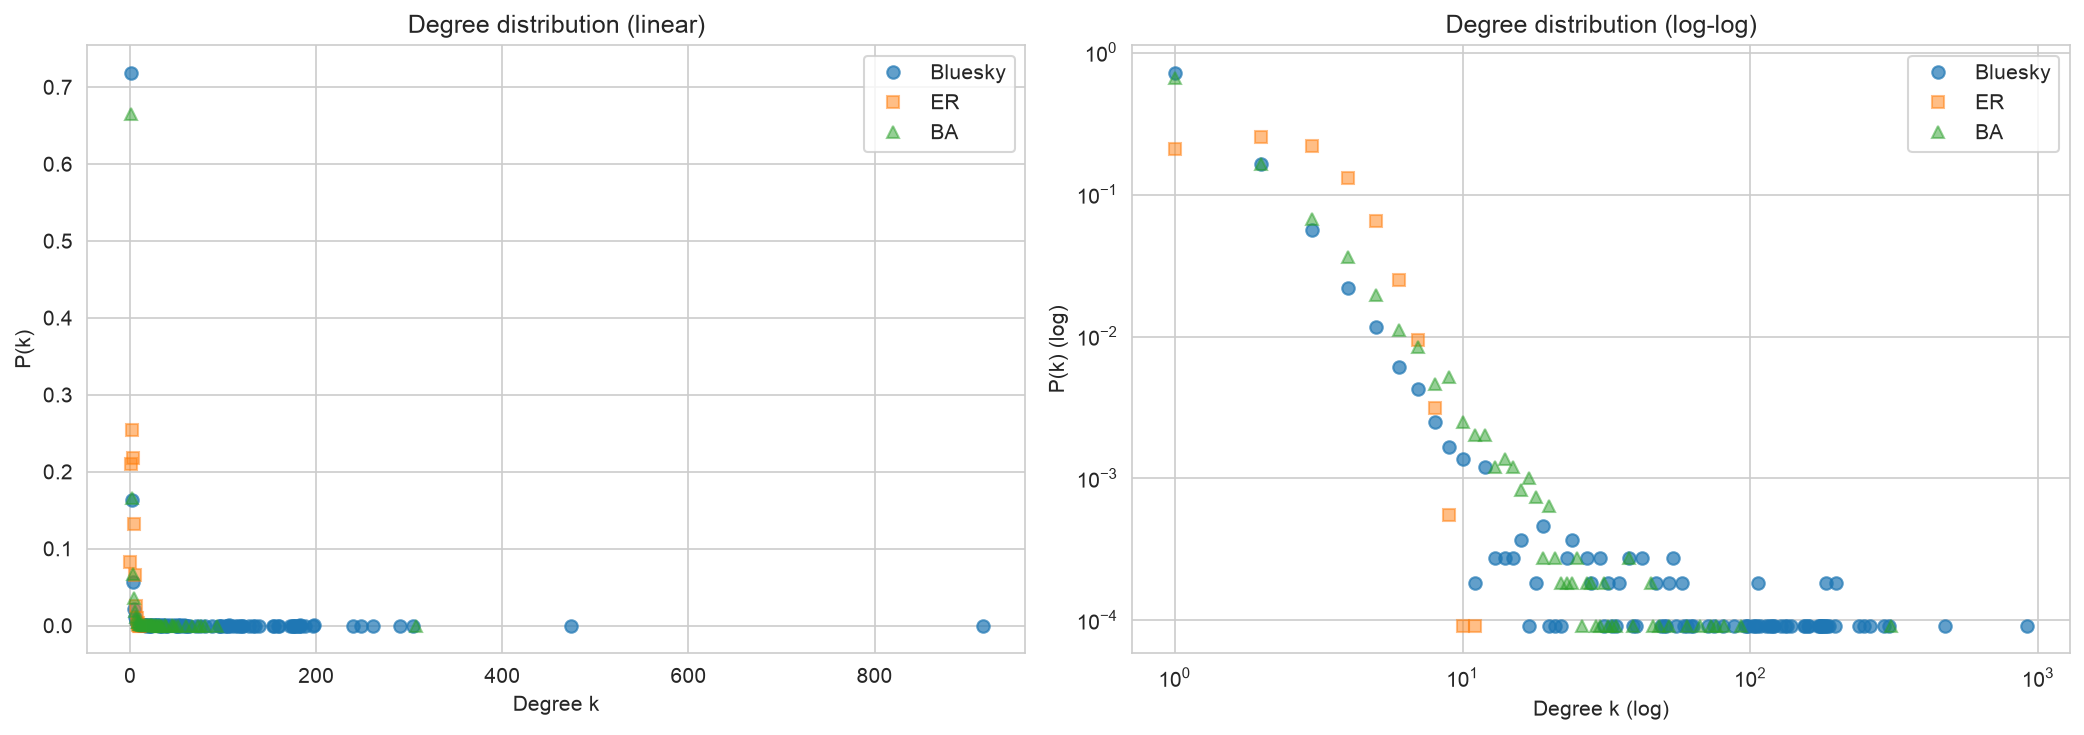
\includegraphics[width=0.85\textwidth]{degree_distribution.png}
  \caption{Degree distribution of Bluesky, ER and BA in linear (left) and log-log scale (right).}
  \label{fig:degdist}
\end{figure*}

\begin{figure}[h]
  \centering
  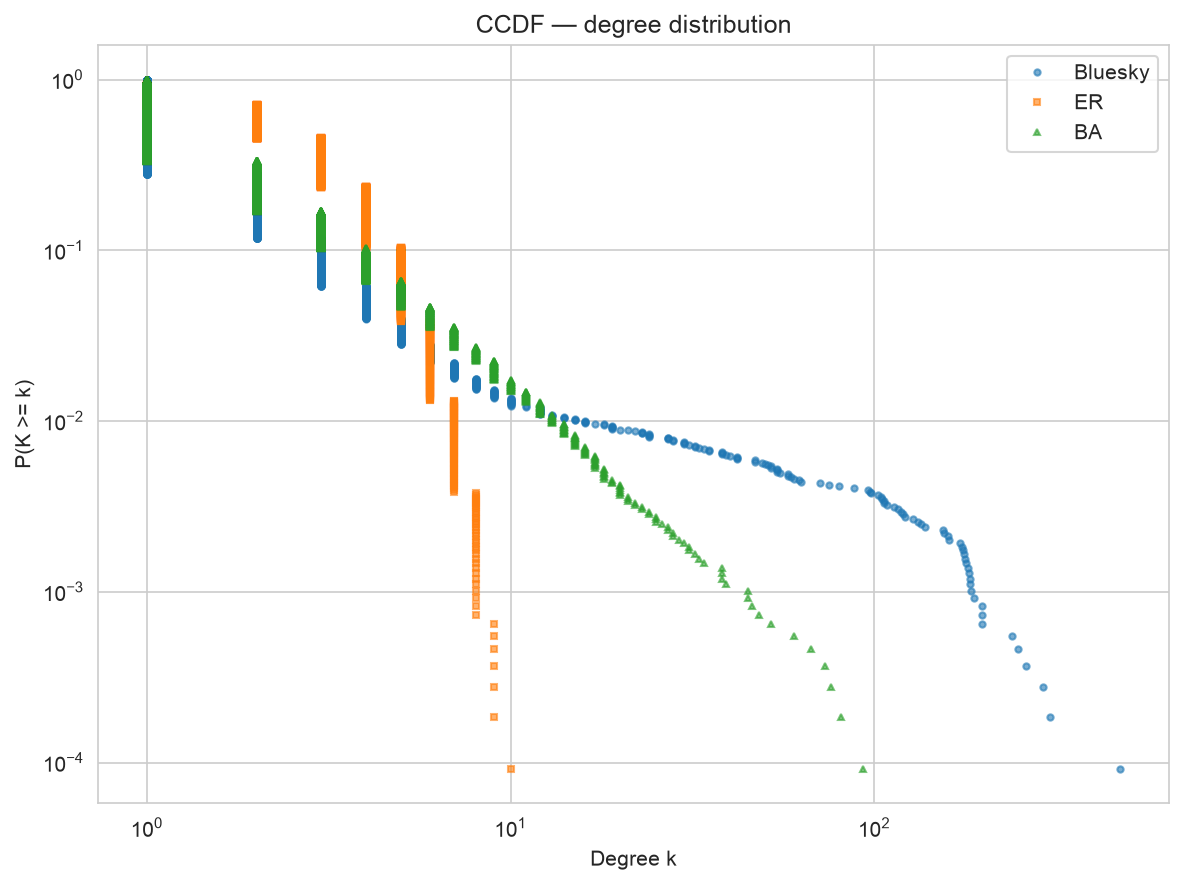
\includegraphics[width=0.9\linewidth]{degree_ccdf.png}
  \caption{CCDF of the degree in log-log scale.}
  \label{fig:ccdf}
\end{figure}

In log-log scale the Bluesky distribution looks almost like a straight line, so we fitted a power law $P(k) \propto k^{-\alpha}$ with the \texttt{powerlaw} library \cite{alstott2014powerlaw}, which uses maximum likelihood \cite{clauset2009powerlaw}. When the library chooses $x_{min}$ automatically (the value that minimises the Kolmogorov-Smirnov distance) it selects $x_{min}=1$, so the fit uses all the nodes, and we obtain $\alpha \approx 2.46$. We then compared the power law with other distributions using the likelihood ratio test of the library ($R>0$ means that the power law fits better). The power law is better than the exponential ($R=9.4$, $p \approx 4.3\cdot10^{-21}$) and the lognormal ($R=13.7$, $p \approx 5.5\cdot10^{-43}$), while the difference with a truncated power law is not significant ($R=0.02$, $p=0.99$), so we cannot say which of the two is better. The ER distribution is concentrated around the mean, as expected for a Poisson distribution, while BA has the typical power-law tail of preferential attachment.

\subsection{Connected Components}
Our network has 65 connected components. The giant component (GCC) contains 10,595 nodes (97.6\%), the second one only 17, and the other 63 components have 243 nodes in total. These are most likely threads whose users do not appear anywhere else in the sample. The ER graph with the same density is much more fragmented: 1,026 components, a GCC with 89.0\% of the nodes and 892 isolated nodes. The BA graph is connected by construction. The following analyses of paths and centralities are computed on the GCC of each graph.

\subsection{Path Analysis}
Since the graphs are not too big, we computed the exact average shortest path length and diameter with a BFS from every node of the GCC. The results are:
\begin{itemize}
\item Bluesky: average distance 5.03, diameter 18;
\item ER: average distance 10.00, diameter 21;
\item BA: average distance 8.86, diameter 23.
\end{itemize}
Our network has the same density as ER, but its distances are about half. The reason is the presence of hubs: many users are connected to the same few accounts, so most paths can go through them. Together with the clustering discussed below, this is the typical behaviour of a small-world network. We have to remember, however, that these hubs are partly created by the way we collected the data.

\subsection{Clustering and Density}
The density of our network is very low ($2.29 \cdot 10^{-4}$) and the same as ER, as expected. The clustering coefficients are reported in Table~\ref{tab:clust}.

\begin{table}[h]
  \caption{Average clustering coefficient and transitivity.}
  \label{tab:clust}
  \begin{tabular}{lrrr}
    \toprule
     & Bluesky & ER & BA \\
    \midrule
    avg. clustering & 0.0325 & 0.0004 & 0 \\
    transitivity & 0.0011 & 0.0007 & 0 \\
    \bottomrule
  \end{tabular}
\end{table}

The average clustering is almost 100 times higher than in ER, so in our network there are more triangles than in a random graph: sometimes, if two users reply to the same account, they also reply to each other. The transitivity, instead, is only slightly higher than in ER. The two measures are different because the average clustering gives the same weight to every node, while the transitivity counts connected triples. Only 740 nodes are part of at least one triangle, and 76.6\% of them have degree 5 or less, so their local clustering is high. On the other hand, 95.8\% of the connected triples are centred on the 50 nodes with the highest degree, whose neighbours are almost never connected to each other (the local clustering of \texttt{ronfilipkowski} is 0.0002). So the triadic closure in our network is present, but weak and limited to a small part of the users.

\subsection{Centrality Analysis}
On the GCC we computed five centrality measures.

\textbf{Degree.} Among the accounts with more neighbours there are journalists, news outlets and political commentators. The top ten are \texttt{ronfilipkowski} (916), \texttt{cortneymckee} (474), \texttt{atrupar.com} (304), \texttt{forbes.com} (290), \texttt{thetnholler} (261), \texttt{reichlinmelnick} (248), \texttt{jonbandit} (239), \texttt{womenriseup2026} (198), \texttt{carlquintanilla} (198) and \texttt{patriottakes} (197).

\textbf{Closeness.} The ranking is similar to the degree one, but not the same: for example \texttt{rbreich} and \texttt{nothoodlum} are in the top six, even if they are not among the nodes with the highest degree.

\textbf{Betweenness.} To save time we estimated it from $k=500$ random source nodes. It is very concentrated: \texttt{ronfilipkowski} has 0.27, more than twice the second node (\texttt{cortneymckee}, 0.12), so a large part of the shortest paths goes through this account.

\textbf{Eigenvector centrality and PageRank.} We computed eigenvector centrality with the power method and PageRank with damping factor 0.85. Eigenvector centrality is almost all on \texttt{ronfilipkowski} (0.70), while all the other nodes are below 0.09: this happens because the score of a node depends on the score of its neighbours, and the neighbours of the biggest hub get most of the value. PageRank, thanks to the random jumps, is more spread over the network.

\begin{figure}[h]
  \centering
  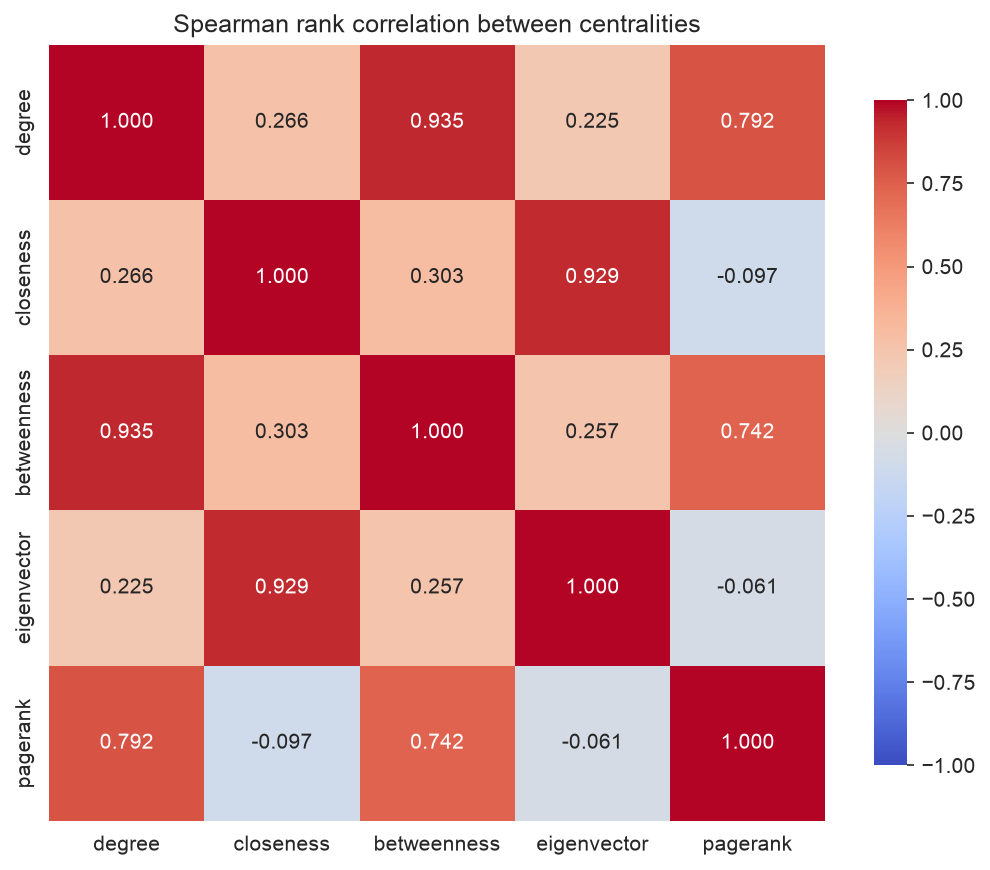
\includegraphics[width=0.85\linewidth]{centrality_correlation.png}
  \caption{Spearman correlation between the five centrality measures on the GCC.}
  \label{fig:cent}
\end{figure}

\textbf{Correlation.} Figure~\ref{fig:cent} shows the Spearman correlation between the measures. Degree, betweenness and PageRank are strongly correlated (between 0.74 and 0.94), so the accounts with more replies are also the ones on most shortest paths. Closeness and eigenvector centrality are strongly correlated with each other (0.93) but only weakly with degree and betweenness (0.23-0.30), and PageRank is not correlated with them ($-0.06$ with eigenvector, $-0.10$ with closeness). The reason is that closeness and eigenvector centrality are high for all the nodes near \texttt{ronfilipkowski}, also the ones with degree 1, while degree and PageRank depend on the number of neighbours of the node itself. In fact, 7,597 nodes of the GCC have degree 1, and 581 of them are connected only to \texttt{ronfilipkowski}: compared with the other degree-1 nodes, these have a higher median closeness (0.24 vs 0.20) and a much higher median eigenvector centrality (0.023 vs 0.0002), but the same PageRank.

\subsection{Comparison with ER and BA}
Overall, our network is sparse, has a giant component with almost all the nodes, a heavy-tailed degree distribution and short distances. ER reproduces the density but not the hubs, the distances and the clustering. BA has hubs and a heavy tail, but with $m=1$ it has fewer edges, longer distances than our network and no triangles. So neither of the two models describes our network well: the hubs are closer to BA, the clustering is higher than both.

\section{Task 1: Community Detection}\label{sec:cd}
Our group has two members, so we had to choose one task of Part 3. We chose community detection because the GCC contains almost all the nodes and because the sentiment of the edges can help us to describe the communities. All the algorithms run on the unweighted GCC ($N=10{,}595$, $M=13{,}263$); the sentiment is only used after, to interpret the results.

\subsection{Algorithms}
We used four algorithms implemented in \texttt{cdlib} \cite{rossetti2019cdlib}:
\begin{itemize}
\item \textbf{Louvain} \cite{blondel2008louvain}: every node is moved to the neighbouring community that gives the largest increase of modularity; then the communities are merged into single nodes and the procedure is repeated.
\item \textbf{Leiden} \cite{traag2019leiden}: an improvement of Louvain that guarantees that every community is connected.
\item \textbf{Infomap} \cite{rosvall2008infomap}: it looks for the partition that gives the shortest description of a random walk on the network. We used the \texttt{-{}-two-level} option to get a flat partition like the other methods.
\item \textbf{Label Propagation} \cite{raghavan2007lpa}: every node takes the most frequent label among its neighbours until the labels do not change. We used the semi-synchronous version \cite{cordasco2010semisync}, which always gives the same result.
\end{itemize}
In a first run with other library versions Infomap and Label Propagation gave different results, because the default options had changed. For this reason we set these options explicitly, fixed the seed of Leiden and wrote the versions of the libraries in the requirements of the repository.

\subsection{Internal Evaluation}
For each partition we computed the number of communities, the size of the largest and of the median community, the Newman-Girvan modularity $Q$, the average conductance (for each community, the fraction of its edges that go outside; lower is better) and the internal edge density (internal edges divided by all the possible pairs of nodes in the community). The results are in Table~\ref{tab:cd}.

\begin{table}[h]
  \caption{Internal evaluation of the four partitions on the GCC.}
  \label{tab:cd}
  \setlength{\tabcolsep}{3pt}
  \begin{tabular}{lrrrrrr}
    \toprule
    Algorithm & \#com. & largest & median & $Q$ & cond. & density \\
    \midrule
    Louvain & 60 & 747 & 165 & 0.819 & 0.15 & 0.02 \\
    Leiden & 60 & 740 & 162 & 0.820 & 0.15 & 0.02 \\
    Infomap & 498 & 592 & 6 & 0.772 & 0.29 & 0.42 \\
    LabelProp & 931 & 863 & 2 & 0.734 & 0.37 & 0.74 \\
    \bottomrule
  \end{tabular}
\end{table}

Louvain and Leiden give very similar results: 60 communities of a few hundred nodes, modularity 0.82 and low conductance. Such a high modularity means that the network has a clear community structure. Infomap and Label Propagation instead find hundreds of small communities (median size 6 and 2), with higher conductance. Their internal density is higher only because small communities have few possible pairs of nodes. Their modularity is also lower, but this comparison is not completely fair, because these two methods do not optimise modularity.

\subsection{Comparison between Algorithms}
To see how similar the partitions are, we computed the Normalized Mutual Information (NMI) and the Adjusted Rand Index (ARI) for every pair of algorithms (Figure~\ref{fig:agree}). Both are 1 when two partitions are identical; ARI is corrected for chance and is close to 0 for random partitions. Louvain and Leiden are very similar (NMI 0.90, ARI 0.85), and so are Infomap and Label Propagation (NMI 0.88, ARI 0.70). Between the two groups the NMI is still quite high (0.76-0.85), while the ARI is lower (0.54-0.64). Since NMI tends to be high when one of the partitions has many small communities, we give more weight to the ARI. Our interpretation is that Infomap and Label Propagation split the communities of Louvain and Leiden into smaller groups, but we did not verify this directly.

\begin{figure}[h]
  \centering
  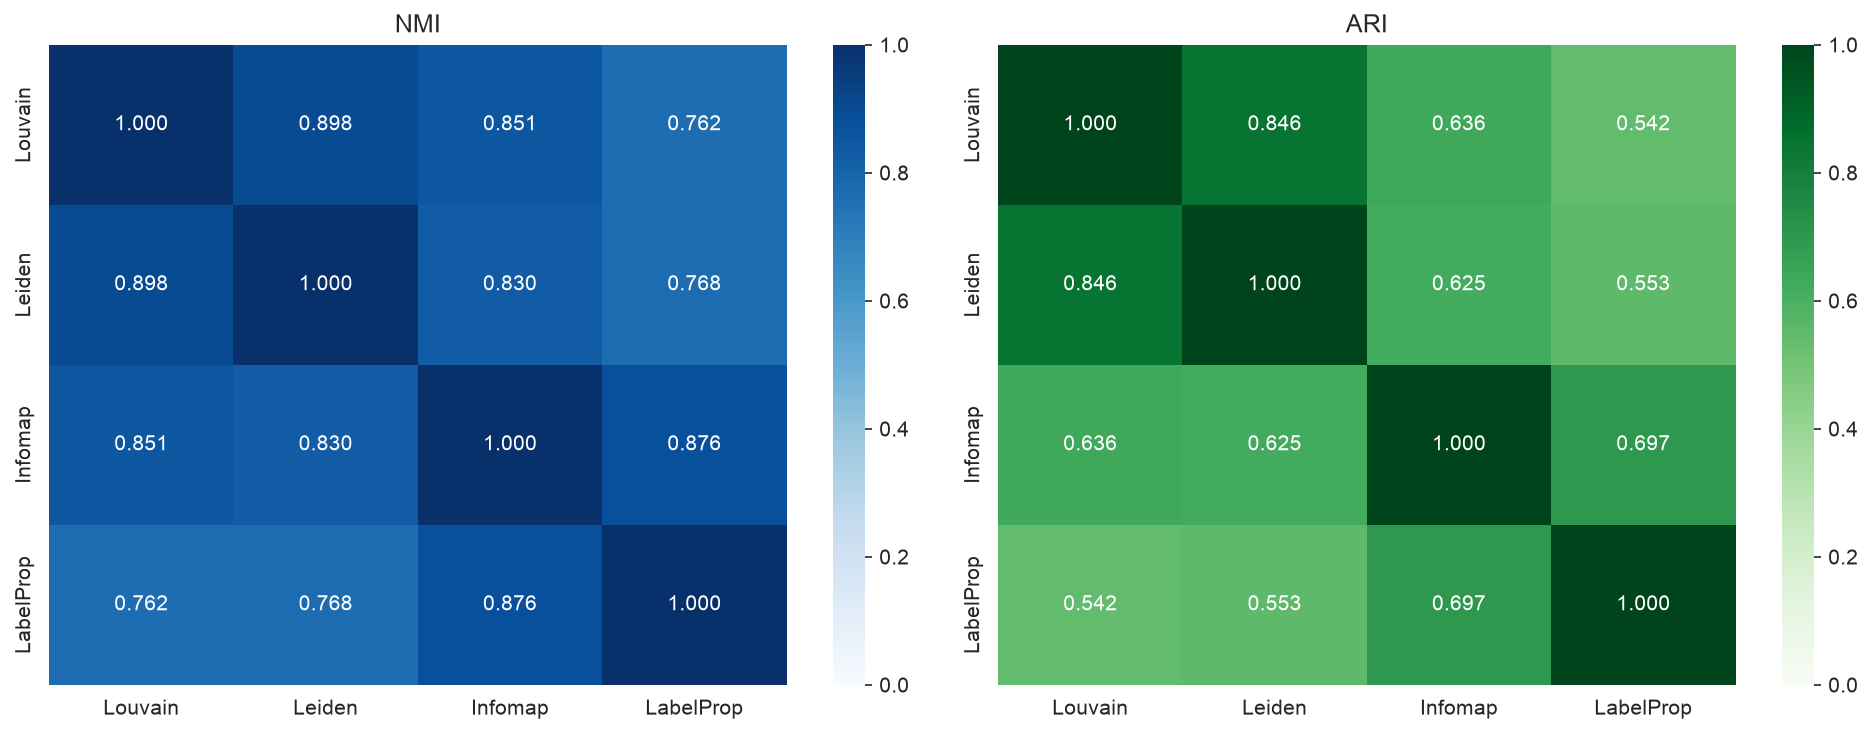
\includegraphics[width=\linewidth]{cd_agreement.png}
  \caption{NMI (left) and ARI (right) between the four partitions.}
  \label{fig:agree}
\end{figure}

\subsection{Communities and Sentiment}
For the interpretation we used the Leiden partition, which has the highest modularity (0.8197, practically the same as Louvain with 0.8186). For each community we looked at the nodes with the highest degree and we computed the mean sentiment of the edges inside the community. Table~\ref{tab:comms} shows some of the largest communities and the only one with a positive mean.

\begin{table}[h]
  \caption{Some Leiden communities: size, fraction of internal edges, mean sentiment of the internal edges and the two nodes with the highest degree.}
  \label{tab:comms}
  \footnotesize
  \setlength{\tabcolsep}{2.5pt}
  \begin{tabular}{rrrl}
    \toprule
    size & internal & sentiment & main nodes \\
    \midrule
    740 & 0.73 & $-0.42$ & \texttt{ronfilipkowski}, \texttt{patriotclyde} \\
    380 & 0.66 & $-0.32$ & \texttt{cortneymckee}, \texttt{h0pe4dfuture} \\
    279 & 0.73 & $-0.42$ & \texttt{carlquintanilla}, \texttt{billkristolbulwark} \\
    274 & 0.69 & $-0.59$ & \texttt{powerbolt}, \texttt{ky-blue17} \\
    257 & 0.75 & $-0.51$ & \texttt{reichlinmelnick}, \texttt{cullenskink} \\
    249 & 0.69 & $-0.55$ & \texttt{atrupar.com}, \texttt{tnsteve.com} \\
    243 & 0.71 & $-0.56$ & \texttt{forbes.com}, \texttt{mayflowerdescendnt} \\
    197 & 0.83 & $+0.08$ & \texttt{phillewis}, \texttt{snelsonus} \\
    \bottomrule
  \end{tabular}
\end{table}

Many of the largest communities contain one of the hubs found in Section~\ref{sec:net}, which is expected since we collected whole threads starting from popular posts. In the 30 largest communities the fraction of edges that stay inside the community goes from 0.65 to 0.89, so users mostly reply to users of the same community.

The sentiment is negative almost everywhere (Figure~\ref{fig:cdsent}): 59 of the 60 communities have a negative mean, and the mean over the communities is $-0.37$ (median $-0.38$). The only exception is the community around \texttt{phillewis}, with a mean of $+0.08$. Moreover, larger communities tend to be more negative (Spearman $\rho=-0.41$, $p<0.01$; Pearson $r=-0.27$, $p=0.04$).

\begin{figure}[h]
  \centering
  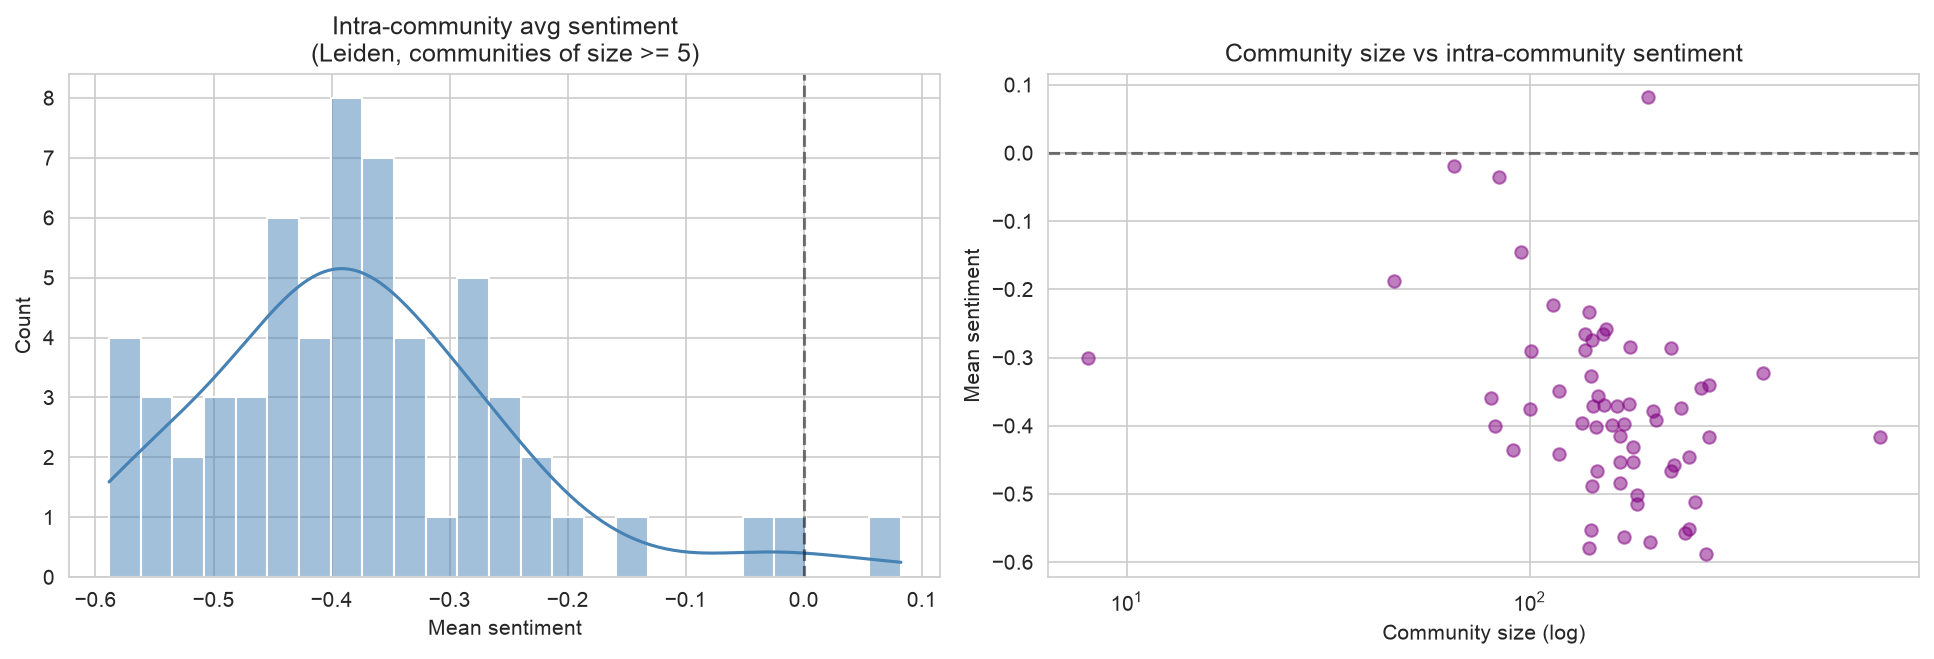
\includegraphics[width=\linewidth]{community_sentiment.png}
  \caption{Left: distribution of the mean sentiment of the Leiden communities. Right: community size and mean sentiment.}
  \label{fig:cdsent}
\end{figure}

These results must be read carefully. A negative sentiment inside a community does not mean that its members are hostile to each other: as said in Section~\ref{sec:data}, the model measures the tone of the text, and users who agree with each other can write negative replies about the same political topic. For this reason the sentiment inside the communities alone does not tell us if they are echo chambers. To study this we need to compare the edges inside the communities with the edges between different communities, which is what we plan to do in the open question.

% ============================================================
% TODO: Task 2 - Open Question (Part 4)
% \section{Task 2: Open Question}\label{sec:oq}
% ============================================================

\section{Discussion}
We built a reply network of 10,855 Bluesky users from political threads. Compared with random graphs of the same size, it has a heavy-tailed degree distribution ($\alpha \approx 2.46$), average distances that are about half of ER, a clustering higher than ER and a clear community structure ($Q \approx 0.82$). Many of the largest communities contain one of the most popular accounts, and almost all the communities have a negative tone.

The main limitation of our work is the sampling. We started from the top posts of three political queries, collected in a single day, and expanded the network from 100 users. This probably makes the hubs bigger and the distances shorter than in the whole platform, and it can also make the sentiment more negative. Other limitations are the BA model with $m=1$, which has fewer edges than our network, the approximated betweenness and the use of a sentiment model trained on Twitter data. Finally, the results of community detection depend on the options and on the versions of the libraries, so we fixed both in our code.

\bibliographystyle{ACM-Reference-Format}
\bibliography{biblio}

\end{document}
